\documentclass[12pt]{article}
\usepackage[a4paper, margin=.30in]{geometry}
%\usepackage{array}
\usepackage{fancybox}

\usepackage{graphicx, subfig, wrapfig, makecell }
\usepackage{multirow}

\newcommand\headerMe[2]{\noindent{}#1\hfill#2}
\renewcommand \thesection{\Roman{section}}

\newcolumntype{M}[1]{>{\raggedright}m{#1}}




\begin{document}

\headerMe{Royaume du Maroc}{année scolaire \emph{2022-2023}}\\
\headerMe{Ministère de l'Éducation nationale, }{  Professeur :\emph{Zakaria Haouzan}}\\
\headerMe{du Préscolaire et des Sports}{Établissement : \emph{Lycée SKHOR qualifiant}}\\

\begin{center}
%Evaluation Diagnostique \\
%Durée 1h45
\hrulefill
\shadowbox{\bf{Rapport de l’évaluation diagnostique }}
\hrulefill\\
\end{center}
%end Headerss------------------------


%__________________Chimie ______________________-
%%%%%%%+_+_+_+_+_+_+_+_+_Partie1
\section[A]{Introduction }
\hspace{0.5cm} Pour constituer une vision globale sur l’état d’avancement des apprenants en Physique chimie, et pour établir le profil de l’ensemble de la classe, une évaluation diagnostique s’impose au début de chaque année scolaire.

Il s’agit de situer les apprenants par rapport aux apprentissages prévus dans le nouveau programme, de détecter leurs pré-requis et pré-acquis, de repérer leurs difficultés d’apprentissage et de déterminer leurs savoirs, savoir-faire et savoir-être relatifs aux différentes compétences requises pour entamer et s’entreprendre les nouveaux apprentissages.

L’évaluation diagnostique en matière Physique chimie pour le niveau 2Bac-SM (2ème année baccalauréat Sciences Mathématiques) , visera les disciplines suivantes : en Physique 3 partie Mécanique , électrodynamique , Optique et Chimie générale .
\section{ Objectifs de l’évaluation diagnostique :}
\begin{itemize}
	\item Etre capable de déterminer les points forts et les points faibles dans les apprentissages antérieurs des apprenants.
	\item Déterminer les difficultés et les obstacles d’apprentissage et motiver les apprenants à les surmonter

	\item Investir les résultats de l’évaluation diagnostique pour planifier les activités de soutien
	\item Adopter ces résultats pour l’orientation et le conseil 

\end{itemize}

\section{Informations générales sur l’évaluation diagnostique :  }
Le tableau ci-dessous et la fiche pédagogique résume la planification de l’évaluation diagnostique et le nombre des apprenants présents :
\begin{center}
  \begin{tabular}{|c|c|c|}
	  \hline
	  La classe & Date de la procédure & Nombre des apprenants présents\\\hline
	  2Bac-SM & 14/09/2022 & 12\\\hline
\end{tabular}
\end{center}

Cette évaluation inclus diverses questions : Questions vrai ou faux et Questions à choix multiples (QCM) dans des Situations problèmes.
\section{Analyse des résultats de l’évaluation diagnostique : }

\begin{center}
  \begin{tabular}{|c|c|c|c|}
	  \hline
La classe & \makecell{Les élèves de niveau faible \\ 0,40} & \makecell{Les élèves moyens \\ ]40,80]}& \makecell{Les élèves brillants \\  ]80,100]} \\\hline
2Bac-SM & \makecell{3 élèves \\ 25\%} & \makecell{7 élèves \\ 59\%}& \makecell{2 élèves \\ 16\%} \\\hline
\end{tabular}
\end{center}

\begin{center}
	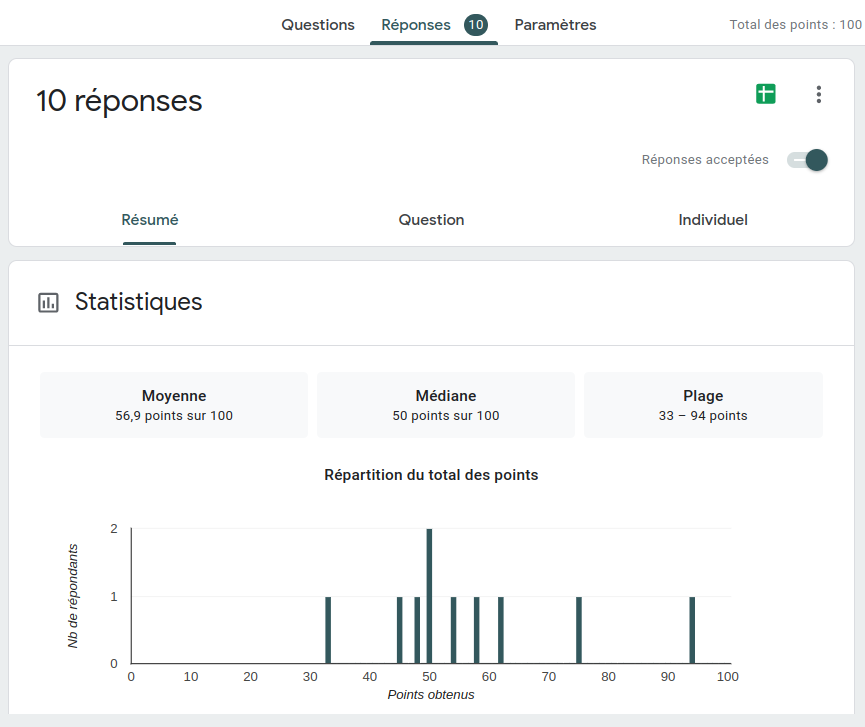
\includegraphics[width=0.5\textwidth]{./img/test-online.png}
\end{center}

Après que les apprenants aient passé ce test et le test online, on peut dire que les résultats obtenus sont en général positifs, mais certaines observations doivent être mentionnées, telles que :

\begin{itemize}
	\item La plupart des apprenants confondent entre les grandeurs physiques et leurs unités dans le système international (Puissance mécanique et électrique, le moment d'une force ...)
	\item Tous les apprenants sauf un ont des problèmes au niveau de la puissance instantanée dans le cas de la rotaion 

	\item  La plupart des apprenants ont oublié les concepts liés à la quantité de matière et la géométrie moléculaire . 
	\item Certains apprenants ont oublié : comment relier le voltmètre et l’ampèremètre pour mesurer la tension et l’intensité de courant,  la loi d’ohm, l’expression de la puissance électrique.
\end{itemize}

\section*{Conclusion : }
\hspace{2cm}En guise de conclusion, les élèves ont  montré  une grande motivation  pou s’améliorer .vis-à-vis des exercices proposés à travers leur engagement, dans le processus de l’enseignement-apprentissage, manifesté par des participations jugées remarquables. Le défi est toujours relevé afin d’aider les élèves en difficulté à suivre le rythme de la classe et de rattraper le temps perdu.

 Pour diminuer les lacunes de certains apprenants au niveau de la matière Physique chimie et perfectionner celle des autres, nous envisageons les propositions suivantes : 
 \begin{itemize}
	 \item Réaliser le soutien (exercices de la physique et la chimie) avec les apprenants en tant que solution d’intervention pour remédier, rattraper, corriger, et combler les lacunes
	 \item Faire des Évaluations Formative au début de chaque chapitre.
	 \item faire un chapitre pour rappeler tous les outils mathématiques dont l’apprenant aura besoin lors des prochaines leçons 

 \end{itemize}

 %\vspace{9cm}
 SIGNATURE DU PROFESSEUR \hspace{3cm} DIRECTEUR  \hspace{3cm} INSPECTEUR

 \vspace{3.85cm}
\emph{Pièces jointes : Evaluation Diagnostique + Fiches pédagogiques.}
\end{document}
